\PassOptionsToPackage{dvipsnames,table}{xcolor}
\documentclass{report}
%%%%%%%%%%%%
% PACKAGES %
%%%%%%%%%%%%
\usepackage[T1]{fontenc}
\usepackage[utf8]{inputenc}
\usepackage{lastpage}

\usepackage[colorinlistoftodos, color=BurntOrange]{todonotes}
\newcommand{\info}[1]{\todo[inline, color=SkyBlue]{#1}}
\newcommand{\question}[1]{\todo[inline, color=SeaGreen]{#1}}

\usepackage[urldate=long]{biblatex}
\addbibresource{references.bib}
\usepackage[hidelinks, linktoc=all]{hyperref}

% Changes the paragraph indentations to newlines
\usepackage{parskip}

\usepackage[a4paper, includeheadfoot, margin=3cm]{geometry}

\usepackage{minted}
\usepackage{xpatch,letltxmacro}
\LetLtxMacro{\cminted}{\minted}
\let\endcminted\endminted
\xpretocmd{\cminted}{\RecustomVerbatimEnvironment{Verbatim}{BVerbatim}{}}{}{}
% \usemintedstyle{manni}
% \usemintedstyle{bw}
% \usemintedstyle{vs}
% \newenvironment{haskell}{\VerbatimEnvironment\begin{center}\begin{minted}[escapeinside=!!]{haskell}}{\end{minted}\end{center}}

\newcommand{\inlinehaskell}[1]{\mintinline[escapeinside=!!, style=bw]{haskell}{#1}}

\usepackage{float}

\usepackage{graphicx}
\graphicspath{ {images} }

\linespread{1.2}

\usepackage[inline]{enumitem}

\usepackage{multicol}
\setlength{\columnsep}{3cm}

\usepackage{datetime}
\newdateformat{monthyeardate}{%
  \monthname[\THEMONTH], \THEYEAR}

%% Fancy Chapter Headers
\usepackage{titlesec}

\newcommand{\chapnumfont}{%     % define font for chapter number
  \usefont{T1}{lmr}{b}{n}%      % choose New Chancery, bold, normal shape
  \fontsize{100}{100}%          % font size 100pt, baselineskip 100pt
  \selectfont%                  % activate font
}
\colorlet{chapnumcol}{gray!75}  % color for chapter number

\titleformat{\chapter}[display]
  {\filleft\bfseries}
  {\filleft\chapnumfont\textcolor{chapnumcol}{\thechapter}}
  {-24pt}
  {\huge}

\titlespacing*{\chapter}{0pt}{-70pt}{40pt}

\usepackage[dvipsnames]{xcolor}

\usepackage[english]{babel}
\usepackage[autostyle]{csquotes}

\usepackage{booktabs}

\usepackage{amssymb}
\usepackage{siunitx}
\usepackage{amsmath}

\usepackage[justification=centering, margin=1cm, belowskip=-10pt, labelfont=bf]{caption}

%%%%%%%%%%%%
% DOCUMENT %
%%%%%%%%%%%%
\begin{document}

\begin{titlepage}
    \fontsize{12pt}{15pt}\selectfont
    \begin{center}
      \vspace*{4cm}
  
      Master's Thesis
  
      \vspace{0.5cm}
  
      {
        \fontsize{20.74pt}{20.74pt}\selectfont
        \parbox[]{13cm} {
          \centering
          Incremental Cata Computation \\ for Generic Data Types
        }
      }
        
      \vspace{1.25cm}
      
      Jort van Gorkum - 6142834 \\
      Computing Science - Programming Technology \\
      Utrecht University \\
      
      \vspace{1.25cm}
      
      Supervisors: \\
      Dr. Wouter Swierstra, Dr. Trevor McDonell \\
      
      \vspace{1cm}
  
      \today
    \end{center}
  \end{titlepage}

\thispagestyle{empty}
\begin{abstract}
\todo[inline]{Make the abstract smaller}
Incremental computation attempts improving performance when the same computation is performed with slightly different input. A specific technique of incremental computation is memoization. Memoization stores the result of a computation and returns the cached result when the same input occurs again. As a result, a large part of memoization becomes dependent on determining if the input is equal to an already cached input. So, when a computation is given a large recursive data structure, the entire data structure needs to be traversed through to determine if it has a cached result. This is inefficient, so, to improve the performance of memoization this paper introduces an incremental algorithm which determines the equality in constant time. This is accomplished by storing hash values/digests, which describe the internal structure, inside the data structure. Furthermore, the incremental algorithm describes how to efficiently update the digests when the data structure changes using a Zipper. The incremental algorithm is also implemented using Datatype-generic programming, to support the class of regular datatypes. At the same time, the usage of the generic implementation stays the same for  the developers as writing the non-incremental algorithm in Haskell. In the end, we show that the performance is better than the non-incremental version with minimal extra memory usage, when correctly tuned with cache policies.
\end{abstract}

% Word limit: 150 - 200 words

\newpage
\thispagestyle{empty}
\tableofcontents

\newpage
\listoftodos

\newpage
\chapter{Introduction}


% Instead, use forward references from the narrative in the introduction. The introduction (including the contributions) should survey the whole paper, and therefore forward reference every important part.

Incremental computation is an approach to improve performance by reusing results of a previously computed result when the both inputs are equal. There are multiple applications where incremental computation has a positive effect on: GUIs (e.g., DOM diffing), spreadsheets, attribute grammar evaluation, etc.  An example, where incremental computation has significant effect on performance, would be computing the Fibonacci sequence.

\begin{minted}{haskell}
fib :: Int -> Int
fib 0 = 0
fib 1 = 1
fib n = fib (n - 2) + fib (n - 1)
\end{minted}

The implementation of the incremental computation for the Fibonacci sequence is called \textit{memoization}. Memoization is a term which is associated with a function that caches the result of the function for the given input. A well-used Haskell library which implements memoization is the \texttt{MemoTrie} library\cite*{hackage2022memotrie}.

This works well when the comparison between inputs can be performed in a small amount of time. However, what if the input of that function is a large recursive data structure, for example a tree. Then, to determine if the memoized inputs and the given input are equal the entire tree needs to be traversed through. To improve the comparison of two data structure, we introduce the use of hash functions. Using hash functions to generate \textit{hash values/digests}, the comparison of two data structures can be performed in constant time.

To store the digests, we label every node in the tree with its corresponding digest. The digest represents the internal structure of itself and its children. This new data structure is called a \textit{Hash Tree} or \textit{Merkle Tree}\cite{merkle1987digital}. Using the digests within the data structure, the comparison can easily be performed by just comparing both digests for equality.

However, what if we want to update a small part of the merkle tree? Then the entire merkle tree needs to be rehashed, while only a small part of changes. The digests of the merkle tree only has to change if the node changes or one of the children nodes changes. In other words, only the nodes that changes and all its parents needs to be updated. To efficiently perform this in Haskell we use a technique named \textit{Zipper}\cite{huet1997zipper}.  

The Zipper keeps track, during the navigation from the root node to a specific node, of the path that has been traversed through the data structure. When the specific node is reached, we update the node with a given function and then update the digests accordingly to the new data structure. Therefore, we only have to update a part of the digest in the data structure.

Unfortunately, when we implement this functionality it only works for a single datatype. When we want to support a different datatype the functionality needs to be copied and reimplemented for that specific datatype. This can become quite cumbersome and error-prone for developers. To support a large class of datatypes for this functionality we introduce \textit{Datatype-Generic programming}.

Datatype-generic programming is a technique to exploit the structure of datatypes to define functions by induction over the type structure. To represent datatypes in a generic, we use pattern functors. Then using datatype-generic programming, we define generic functionality for: computing the digests of the data structure, storing the digests inside the data structure, a generic zipper, and, finally functionality for computing the result for a given function and cache with intermediate results. 

However, this does mean that the given function which computes a result needs to use the representation types. The representation types are quite verbose and the extension cannot be a drop-in replacement for existing functionality. To make it easier for developers to use, we introduce \textit{Pattern synonyms}\cite*{pickering2016pattern}. Pattern synonyms add an abstraction over patterns, which can be used to simplify the case expressions used in the given function, making the functionality almost a drop-in extension (we only need to add an underscore to the data constructors). 

Finally, to keep the cache from growing too large for the available amount of memory, we show multiple policies, so that the developer can choose the best policy for their use-case. The policy can be focused on recency, frequency, computational cost or a combination of the previously mentioned metrics.

\section{Contributions}

In summary, the main contributions of the Thesis are the following:

\begin{itemize}
    \item We define an algorithm for incremental computation over recursive data structures. The algorithm uses hashes for comparing if data structures are equal in constant time and a Zipper to efficiently update the recursive data structure without rehashing the entire data structure.
    \item We use datatype-generic programming to write a generic version of the algorithm, to support a large class of datatypes, namely \textit{regular datatypes}.
    \item We use pattern synonyms, to make the developer experience the same as implementing a non-incremental algorithm.
    \item We define cache addition policies and cache replacement policies to optimize the performance/memory usage for different use-cases.
\end{itemize}


% \section{Current Situation}
% \question{Familiar with MemoTrie?}
% \begin{itemize}
%   \item \href{https://hackage.haskell.org/package/MemoTrie}{MemoTrie}
%   \begin{itemize}
%     \item MemoTrie is memoization of a function, compared to this Thesis project which performs memoization on a recursive data structure.
%     \item Does not use hashes to compare the inputs for equality, but uses sums of products to represent the datatypes. This results in keys that fluctuate in size, which can become quite large, while the hashes are of a constant size.
%     \item Has to traverse the complete data structure for equality. This paper the equality check is constant and efficiently updated when data structure changes.
%   \end{itemize}
%   \item \href{https://monospacedmonologues.com/2022/01/memotries/}{Blog MemoTrie}
%   \item \href{https://www.cs.uu.nl/research/techreps/repo/CS-2009/2009-024.pdf}{Pull-Ups, Push-Downs, and Passing It Around.
%   Exercises in Functional Incrementalization}
%   \begin{itemize}
%     \item -
%   \end{itemize}
%   \item \href{https://citeseerx.ist.psu.edu/viewdoc/download?doi=10.1.1.43.3272&rep=rep1&type=pdf}{Memo funtions, polytypially!}
%   \begin{itemize}
%     \item Is the paper version of the MemoTrie implementation
%   \end{itemize}
% \end{itemize}

% \newpage
% \chapter{Introduction}

\todo[inline]{Write more context}
\todo[inline]{Add a problem statement}

\todo[inline]{Add why my thesis is unique}

Incremental computation is an approach to improve performance by computing only the result of the changed parts of the input, instead of computing the entire result. To determine what parts of the input has changed, we provide a \textit{Zipper} which can be used by the user to efficiently update the previous input to a new input and keeps track of the changes to the input. As a result, we know which parts of the input stays the same. Therefore, we can reuse the results of a previously performed computation for the same input\footnote{The technique for reusing results based on input is called \textit{memoization}}.   

The task of implementing incremental computation for Haskell is explained in Chapter \ref*{chap-spec-impl}. However, the task for implementing incremental computation for multiple datatypes, becomes repetitive and error-prone. To prevent writing implementations for every datatype, we use datatype-generic programming. Datatype-generic programming is a technique that uses the structure of a datatype to define functions for a large class of datatypes, which is explained in more detail in Chapter \ref*{chap-dat-gen-program}. Then, using the Haskell generics library \texttt{regular}, we implement the generic version. In Chapter \ref*{chap-gen-impl}, the generic implementation is explained and additionally describe: complexity, different garbage collection strategies and different data structures for storing results. 

To illustrate how the incremental computation functionality is used, an example is presented which implements the \textbf{max-path-sum} in a non-incremental and an incremental manner. The max-path-sum function traverses through a tree and returns the sum of the path with the highest value. For the example, we first define the definition of a tree and an example tree which is used as input for the max-path-sum. Then, the non-incremental function (\inlinehaskell{maxPathSum}) is implemented, by returning the value for the leaf; and for the node recursively calling the children and determine the highest value between the children and adding it to its own value.

\begin{minted}{haskell}
data BinTree = Leaf Int
             | Node BinTree Int BinTree 
             
exampleTree :: BinTree    
exampleTree = Node (Node (Leaf 8) 7 (Leaf 1)) 3 (Node (Leaf 5) 4 (Leaf 2))

-- The non-incremental implementation of max-path-sum
maxPathSum :: BinTree -> Int
maxPathSum (Leaf x)     = x
maxPathSum (Node l x r) = x + max (maxPathSum l) (maxPathSum r)

> maxPathSum exampleTree
    18

> let exampleTree' = update (const (Leaf 6)) [Bttm] exampleTree

> maxPathSum exampleTree'
    16
\end{minted}

The incremental implementation, first adds hashes to the input which represent the internal data structure to the data structure (also known as a \textit{merkle tree}). This is used to efficiently check what parts of the input has changed. Then, the initial computation is performed which gives the result and a map of all the intermediate results. Next, the tree gets updated, in this case the bottom left leaf (\inlinehaskell{Leaf 8}) is replaced with \inlinehaskell{Leaf 6}. Finally, the updated tree is recomputed reusing the previously computed results. As a result, the complete right side of the root node did not have to be recomputed, because it stayed the same.

\todo[inline]{Add the explanation of that we use the Zipper for updating the Tree}

\begin{minted}{haskell}
-- The incremental implementation of max-path-sum
incMaxPathSum :: BinTree -> Int
incMaxPathSum (Leaf_ x)     = x
incMaxPathSum (Node_ l x r) = x + max l r

-- Add hashes to data structure
> let merkleTree = merkle exampleTree

-- Initial computation
> let (y, m) = cataMerkle incMaxPathSum (merkleTree)
    (18, { "6dd": 18, "5df": 15, "fa0": 8, "8d0": 1, "f3b": 9, "84b": 5
         , "1ad": 2 })

-- Update Tree
> let merkleTree' = update (const (merkle (Leaf 6))) [Bttm] merkleTree

-- Incremental computation
> cataMerkleMap incMaxPathSum m (merkleTree')
    (16, { "6dd": 18, "5df": 15, "fa0": 8, "bbd": 16, "91c": 13, "3af": 6
         , "8d0": 1, "f3b": 9, "84b": 5, "1ad": 2 })
\end{minted}

\section{Contributions}

The main contributions of the Thesis are the following:

\begin{itemize}
    \item We define an algorithm for incremental computation over recursive data structures. The algorithm uses hashes for comparing if the data structures are equal in a constant time and a Zipper to efficiently update the recursive data structure without rehashing the entire data structure.
    \item We use datatype-generic programming to write a generic version of the algorithm, to support a large class of datatypes, namely \textit{regular datatypes}.
    \item We use pattern synonyms, to make the developer experience the same as implementing a non-incremental algorithm.
    \item We define cache addition policies and cache replacement policies to optimize the performance/memory usage for different use-cases.
\end{itemize}


\newpage
\chapter{Specific Implementation}
\label{chap-spec-impl}

\begin{minted}{haskell}
data Tree a = Leaf a
            | Node (Leaf a) a (Leaf a)
\end{minted}

\begin{minted}{haskell}
sumTree :: Tree Int -> Int
sumTree (Leaf x)     = x
sumTree (Node l x r) = x + (sumTree l) + (sumTree r)
\end{minted}

Computing a value of a data structure can easily be defined in Haskell, but every time there is a small change in the \texttt{Tree}, the entire \texttt{Tree} needs to be recomputed. This is inefficient, because most of the computations have already been performed in the previous computation. 

To prevent recomputation of already computed values, the technique memoization is introduced. Memoization is a technique where the results of computational intensive tasks are stored and when the same input occurs, the result is reused. 

The comparison of two values in Haskell is done with the \texttt{Eq} typeclass, which implements the equality operator \inlinehaskell{(==) :: a -> a -> Bool}. So, an example implementation of the \texttt{Eq} typeclass for the \texttt{Tree} datatype would be:

\begin{minted}{haskell}
instance Eq a => Eq (Tree a) where
  Leaf x1       == Leaf x2       = x1 == x2
  Node l1 x1 r1 == Node l2 x2 r2 = x1 == x2 && l1 == l2 && r1 == r2
  _             == _             = False
\end{minted}

The problem with using this implementation of the \texttt{Eq} typeclass for Memoization is that for every comparison of the \texttt{Tree} datatype the equality is computed. This is inefficient because the equality implementation has to traverse the complete \texttt{Tree} data structure to know if the \texttt{Tree}'s are equal. 

To efficiently compare the \texttt{Tree} datatypes, we need to represent the structure in a manner which does not lead to traversing to the complete \texttt{Tree} data structure. This can be accomplished using a \texttt{hash} function. A hash function is a process of transforming a data structure into an arbitrary fixed-size value, where the same input always generates the same output. 

One of the disadvantages of using hashes is \textit{hash collisions}. Hash collisions happen when two different pieces of data have the same hash. This is because a hash function has a limited amount of bits to represent every possible combination of data. Using the formula $p = \epsilon^{\frac{-k(k-1)}{2N}}$ from \citetitle{hashcoll2011}\cite{hashcoll2011}, we can calculate a $50\%$ chance of getting a hash collision with a collection of $k$. The hash function CRC-32 needs a collection of 77163 hash values. The hash function MD5 needs a collection of $\num{5.06e9}$ hash values. And, the hash function SHA-1 needs a collection of $\num{1.42e24}$ hash values. As a result of, we can say that for most popular hash functions, that the hash collisions are negligible.

\todo[inline]{Add which hash is ultimately chosen}

\begin{minted}{haskell}
class Hashable a where
  hash :: a -> Hash

instance Hashable a => Hashable (Tree a) where
  hash (Leaf x)     = concatHash [hash "Leaf", hash x]
  hash (Node l x r) = concatHash [hash "Node", hash x, hash l, hash r]
\end{minted}

The hashes can then be used to efficiently compare two \texttt{Tree} data structures, without having to traverse the entire \texttt{Tree} data structure. To keep track of the intermediate results of the computation, we store the results in a \texttt{Map}. A \texttt{Map}, also known as a dictionary, is an implementation of mapping a key to a value. In our next example the \texttt{Hash} is the key and the value is the intermediate result.

\begin{minted}{haskell}
sumTreeInc :: Tree Int -> (Int, Map Hash Int)
sumTreeInc l@(Leaf x)     = (x, insert (hash l) x empty)
sumTreeInc n@(Node l x r) = (y, insert (hash n) y (ml <> mr))
  where
    y = x + xl + xr
    (xl, ml) = sumTreeInc l
    (xr, mr) = sumTreeInc r
\end{minted}

Then after the first computation over the entire \texttt{Tree}, we can recompute the \texttt{Tree} using the previously created \texttt{Map}. Thus, when we recompute the \texttt{Tree}, we first look in the \texttt{Map} if the computation has already been performed then return the result. Otherwise, compute the result and store it in the \texttt{Map}.

\begin{minted}{haskell}
sumTreeIncMap :: Map Hash Int -> Tree Int -> (Int, Map Hash Int)
sumTreeIncMap m l@(Leaf x) = case lookup (hash l) m of
  Just x  -> (x, m) 
  Nothing -> (x, insert (hash l) x empty)
sumTreeIncMap m n@(Node l x r) = case lookup (hash n) m of
  Just x  -> (x, m)
  Nothing -> (y, insert (hash n) y (ml <> mr))
    where
      y = x + xl + xr
      (xl, ml) = sumTreeIncMap m l
      (xr, mr) = sumTreeIncMap m r
\end{minted}

Generating a hash for every computation over the data structure is time-consuming and unnecessary, because most of the \texttt{Tree} data structure stays the same. The work of \citeauthor{miraldo2019efficient}\cite{miraldo2019efficient} inspired the use of the Merkle Tree. A Merkle Tree is a data structure which integrates the hashes within the data structure.

\section{Merkle Tree (\texttt{TreeH})}
First we introduce a new datatype \texttt{TreeH}, which contains a \texttt{Hash} for every constructor in \texttt{Tree}. Then to convert the \texttt{Tree} datatype into the \texttt{TreeH} datatype, the structure of the Tree is hashed and stored into the datatype using the \texttt{merkle} function.

\begin{minted}{haskell}
data TreeH a = LeafH Hash a
             | NodeH Hash (Leaf a) a (Leaf a)
\end{minted}

\begin{minted}{haskell}
merkle :: Tree Int -> TreeH Int
merkle l@(Leaf x) = LeafH (hash l) x
merkle (Node l x r) = NodeH h l' x r'
  where
    h = hash ["Node", x, getHash l', getHash r']
    l' = merkle l
    r' = merkle r
\end{minted}

The precomputed hashes can then be used to easily create a \texttt{Map}, without computing the hashes every time the \texttt{sumTreeIncH} function is called.

\begin{minted}{haskell}
sumTreeIncH :: TreeH Int -> (Int, Map Hash Int)
sumTreeIncH (LeafH h x)     = (x, insert h x empty)
sumTreeIncH (NodeH h l x r) = (y, insert h y (ml <> mr))
  where
    y = x + xl + xr
    (xl, ml) = sumTreeInc l
    (xr, mr) = sumTreeInc r
\end{minted}

The problem with this implementation is, that when the \texttt{Tree} datatype is updated, the entire \texttt{Tree} needs to be converted into a \texttt{TreeH}, which is linear in time. This can be done more efficiently, by only updating the hashes which are impacted by the changes. Which means that only the hashes of the change and the parents need to be updated. 

The first intuition to fixing this would be using a pointer to the value that needs to be changed. But because Haskell is a functional programming language, there are no pointers. Luckily, there is a data structure which can be used to efficiently update the data structure, namely the Zipper\cite{huet1997zipper}.

\section{Zipper}

% \question{Add a visual example?}

The Zipper is a technique of representing a data structure by keeping track of how the data structure is being traversed through. The Zipper was first described by \citeauthor{huet1997zipper}\cite{huet1997zipper} and is a solution for efficiently updating pure recursive data structures in a purely functional programming language (e.g., Haskell). This is accomplished by keeping track of the downward current subtree and the upward path, also known as the \textit{location}. 

To keep track of the upward path, we need to store the path we traverse to the current subtree. The traversed path is stored in the \texttt{Cxt} datatype. The \texttt{Cxt} datatype represents three options the path could be at: the \texttt{Top}, the path has traversed to the left (\texttt{L}), or the path has traversed to the right (\texttt{R}).

\begin{minted}{haskell}
data Cxt a = Top
           | L (Cxt a) (Tree a) a
           | R (Cxt a) (Tree a) a

type Loc a = (Tree a, Cxt a)

enter :: Tree a -> Loc a
enter t = (t, Top)           
\end{minted}

Using the \texttt{Loc}, we can define multiple functions on how to traverse through the \texttt{Tree}. Then, when we get to the desired location in the \texttt{Tree}, we can call the \texttt{modify} function to change the \texttt{Tree} at the current location.

\begin{minted}{haskell}
left :: Loc a -> Loc a
left (Node l x r, c) = (l, L c r x)

right :: Loc a -> Loc a
right (Node l x r, c) = (r, R c l x)

up :: Loc a -> Loc a
up (t, L c r x) = (Node t x r, c)
up (t, R c l x) = (Node l x t, c)

modify :: (Tree a -> Tree a) -> Loc a -> Loc a
modify f (t, c) = (f t, c)
\end{minted}

Eventually, when every value in the \texttt{Tree} has been changed, the entire \texttt{Tree} can then be rebuilt using the \texttt{Cxt}. By recursively calling the \texttt{up} function until the top is reached, the current subtree gets rebuilt. And when the top is reached, the entire tree is then returned.

\begin{minted}{haskell}
leave :: Loc a -> Loc a
leave l@(t, Top) = l
leave l = top (up l)
\end{minted}

\subsection{Zipper \texttt{TreeH}}

The implementation of the Zipper for the \texttt{TreeH} datatype is the same as for the \texttt{Tree} datatype. However, the \texttt{TreeH} also contains the hash of the current and underlying data structure. Therefore, when a value is modified in the \texttt{TreeH}, all the parent nodes of the modified value needs to be updated. 

The \texttt{updateLoc} function modifies the value at the current location, then checks if the location has any parents. If the location has any parents, go up to that parent, update the hash of that parent and recursively update the parents hashes until we are at the top of the data structure. Otherwise, return the modified locations, because all the other hashes are not affected by the change. 

\begin{minted}{haskell}
updateLoc :: (TreeH a -> TreeH a) -> Loc a -> Loc a
updateLoc f l = if top l' then l' else updateParents (up l')
    where
        l' = modify f l

        updateParents :: Loc a -> Loc a
        updateParents (Loc x Top) = Loc (updateHash x) Top
        updateParents (Loc x cs)  = updateParents $ up (Loc (updateHash x) cs)
\end{minted}

Then, the \texttt{update} function can be defined using the \texttt{updateLoc} function, by first traversing through the data structure with the given directions. Then modifying the location using the \texttt{updateLoc} function and then leave the location and the function results in the updated data structure.

\begin{minted}{haskell}
update :: (TreeH a -> TreeH a) -> [Loc a -> Loc a] -> TreeH a -> TreeH a 
update f dirs t = leave $ updateLoc f l'
    where
        l' = applyDirs dirs (enter t)
\end{minted}

\newpage
\chapter{Datatype-Generic Programming}
\label{chap-dat-gen-program}

\todo[inline]{Compare paper \citetitle{van2008lightweight}}

The implementation in Chapter \ref{chap-spec-impl} is an efficient implementation for incrementally computing the summation over a \texttt{Tree} datatype. However, when we want to implement this functionality for a different datatype, a lot of code needs to be copied while the process remains the same. This results in poor maintainability, is error-prone and is in general boring work.

An example of reducing manual implementations for datatypes is the \textit{deriving} mechanism in Haskell. The built-in classes of Haskell, such as \texttt{Show, Ord, Read}, can be derived for a large class of datatypes. However, deriving is not supported for custom classes. Therefore, we use \textit{Datatype-Generic Programming}\cite*{gibbons2006datatype} to define functionality for a large class of datatypes.

In this chapter, we introduce Datatype-Generic Programming, also known as \textit{generic programming} or \textit{generics} in Haskell, as a technique that uses the structure of a datatype to define functions for a large class of datatypes. This prevents the need to write the previously defined functionality for every datatype.

\section{Introduction}
There are multiple generic programming libraries, however to demonstrate the workings of generic programming we will be using a single library as inspiration, named \texttt{regular}\cite*{regular2022}. Here the generic representation of a datatype is called a \textit{pattern functor}. A pattern functor is a stripped-down version of a data type, by only containing the constructor but not the recursive structure. The recursive structure is done explicitly by using a fixed-point operator. 

First, the pattern functors defined in \texttt{regular} are 5 core pattern functors and 2 meta information pattern functors. The core pattern functors describe the datatypes. The meta information pattern functors only contain information (e.g., constructor name) but not any structural information.

\question{What do you call the datatypes which combine into a pattern functor?}

\begin{minted}{haskell}
data U r         = U                 -- Empty constructors
data I r         = I r               -- Recursive call
data K a r       = K a               -- Constants
data (f :+: g) r = L (f r) | R (g r) -- Sums (Choice)
data (f :*: g) r = (f r) :*: (g r)   -- Products (Combine)
\end{minted}

The conversion from regular datatypes into pattern functors is done by the \texttt{Regular} type class. The \texttt{Regular} type class has two functions. The \texttt{from} function converts the datatype into a pattern functor and the \texttt{to} function converts the pattern functor back into a datatype. In \texttt{regular}, the pattern functor is represented by a type family. Then using the \texttt{Regular} conversion to a pattern functor, we can write the \texttt{Tree} datatype from Chapter \ref{chap-spec-impl} as:

\begin{minted}{haskell}
type family PF a :: * -> *

class Regular a where
  from :: a -> PF a a
  to   :: PF a a -> a

type instance PF (Tree a) = K a                -- Leaf
                         :+: (I :*: K a :*: I) -- Node

class Regular (Tree a) where
  from (Leaf x)     = L (K x)
  from (Node l x r) = R (I l :*: K x :*: I r)                 

  to (L (K x))                 = Leaf x
  to (R (I l :*: K x :*: I r)) = Node l x r
\end{minted}

To demonstrate the workings of generic programming, we are going to implement a simple generic function which determines the length of an arbitrary datatype. First, we define the length function within a type class. The type class is used, to define how to determine the length for every pattern functor \texttt{f}. 

\begin{minted}{haskell}
class GLength f where
  glength :: (a -> Int) -> f a -> Int
\end{minted}

Writing instances for the empty constructor \texttt{U} and the constants \texttt{K} is simple because both pattern functors return zero. The \texttt{U} pattern functor returns zero, because it does not contain any children. The \texttt{K} pattern functor returns zero, because we do not count constants for the length. 

\begin{minted}{haskell}
instance GLength U where
  glength _ _ = 0

instance GLength (K a) where
  glength _ _ = 0
\end{minted}

The instances for sums and products pattern functors are quite similar. The sums pattern functor recurses into the specified choice. The product pattern functor recurses in both constructors and combines them.

\begin{minted}{haskell}
instance (GLength f, GLength g) => GLength (f :+: g) where
  glength f (L x) = glength f x
  glength f (R x) = glength f x

instance (GLength f, GLength g) => GLength (f :*: g) where
  glength f (x :*: y) = glength f x + glength f y
\end{minted}

The instance for the recursive call \texttt{I} needs an additional argument. Because, we do not know the type of \texttt{x}, so an additional function (\inlinehaskell{f :: a -> Int}) needs to be given which converts \texttt{x} into the length for that type.

\begin{minted}{haskell}
instance GLength I where
  glength f (I x) = f x
\end{minted}

Then using the \texttt{GLength} instances for all pattern functors, a function can be defined using the generic length function. By first, converting the datatype into a generic representation, then calling \texttt{glength} given recursively itself, and for every recursive call increase the length by one. 

\begin{minted}{haskell}
length :: (Regular a, GLength (PF a)) => a -> Int
length = 1 + glength length (from x)
\end{minted}

\begin{minted}{haskell}
> length [1, 2, 3]
    3
> length (Node (Leaf 1) 2 (Leaf 3))
    3
> length {"1": 1, "2": 2, "3": 3}
    3
\end{minted}

\subsection{Explicit recursion}
\label{sec-explicit-recursion}

% There are two ways to define the representation of values. Those that have information about which fields of the constructors of the datatype in question are recursive versus those that do not.

The previous implementation of the \texttt{length} function is implemented for a shallow representation. A shallow representation means that the recursion of the datatype is not explicitly marked. Therefore, we can only convert one layer of the value into a generic representation using the \texttt{from} function. 

Alternatively, by marking the recursion of the datatype explicitly, also called the deep representation, the entire value can be converted into a generic representation in one go. To mark the recursion, a fixed-point operator (\texttt{Fix}) is introduced. Then, using the fixed-point operator we can define a from function that given the pattern functors have an instance of Functor\footnote{The Functor instances for the pattern functors can be found in Section \ref{app-inst-functor-patfun}}, return a generic representation of the entire value.

\begin{minted}{haskell}
data Fix f = In { unFix :: f (Fix f) }

deepFrom :: (Regular a, Functor (PF a)) => a -> Fix (PF a)
deepFrom = In . fmap deepFrom . from
\end{minted}

Subsequently, we can define a \texttt{cata} function which can use the explicitly marked recursion by applying a function at every level of the recursion. Then using the \texttt{cata} function we can define the same \texttt{length} function as in the previous section, but just in a single line. However, this deep representation does come at the cost that the implementation is less efficient than the shallow representation. 

\begin{minted}{haskell}
cata :: Functor f => (f a -> a) -> Fix f -> a
cata = f . fmap (cata f) . unFix

length' :: (Regular a, GLength (PF a), Functor (PF a), Foldable (PF a)) 
        => a -> Int
length' = cata ((1+) . sum) . deepFrom
\end{minted}

\section{Sums of Products}
\todo[inline]{Add a description of what a universe is}

A different way of describing datatypes in a generic representation, besides pattern functors, are \textit{Sums of Products}\cite{vries2014sums} (SOP). SOP is a generic representation with additional constraints which more faithfully reflects the Haskell datatypes: each datatype is a single n-ary sum, where each component of the sum is a single n-ary product. The SOP universe is described using \textit{codes} of kind \texttt{[[*]]}. The outer list describes an n-ary sum, representing the choice between constructors and each inner list an n-ary products, representing the constructor arguments.  The code of kind \inlinehaskell{[[*]]} can then be interpreted to describe Haskell datatypes of kind \inlinehaskell{*}. To define a code, the tick mark \inlinehaskell{`} is used to lift the list to a type-level. 

\begin{minted}{haskell}
Code (Tree a) = `[`[a], `[Tree a, a, Tree a]]
\end{minted}

The usage of SOP has a positive effect on expressing generic functions easily or at all. Additionally, the SOP completely divides the structural representation from the metadata. As a result, you do not have to deal with metadata while writing generic functions. However, the additional constraints on the generic representation makes the SOP universe size comparatively bigger than pattern functors. Therefore, it is more complex to extend the SOP than for pattern functors.

% \begin{itemize}
%     \item While many of the libraries that are
%     commonly in use today represent datatypes as arbitrary combinations of binary sums and products, SOP reflects the structure of datatypes more faithfully: each datatype is a single n-ary sum, where each component of the sum is a single n-ary product.
%     \item A major plus of the SOP view is that it allows separating function-specific metadata from the main structural representation and recombining this information later.
%     \item In this paper, we introduce a view (which we call SOP) which is based on a single, n-ary, sum, where each component of the sum is a single, n-ary, product.
%     \item The SOP view also takes a very interesting approach to metadata. In most generic views, metadata is intertwined with the structural representation, which means that every generic function has to deal with it in some way—even if it is just ignored, as in the M1 case for \texttt{garities} shown above. Furthermore, metadata sometimes leads to additional implicit assumptions about the shape of the data.
%     \item In the SOP view, metadata is completely independent from the data representation. This means that functions which do not need it, don't have to deal with it; conversely, it also means that we can easily define application-specific metadata, i.e., type-directed additional information that “configures” how a particular generic function should behave.
%     \item The tick marks are used to explicitly indicate that we mean the promoted type.
%     \item The fundamental idea of the SOP universe is that the kind of codes is a (promoted) list of list of types, written [[*]]. The goal of the universe is to provide descriptions of Haskell datatypes (of kind *)
% \end{itemize}



\subsection{Mutually recursive datatypes}
A large class of datatypes is supported by the previous section, namely \textit{regular} datatypes. Regular datatypes are datatypes in which the recursion only goes into the same datatype. However, if we want to support the abstract syntax tree of many programming languages, we need to support datatypes which can recurse over different datatypes, namely mutually recursive datatypes.

\begin{minted}{haskell}
data Tree a = Empty 
            | Node (a, Forest a)

data Forest a = Nil
              | Cons (Tree a) (Forest a)
\end{minted}

To support mutually recursive datatypes, we need to keep track of which recursive position points to which datatype. This is accomplished by using \textit{indexed fixed-points}\cite{yakushev2009generic}. The indexed fixed-points works by creating a type family $\varphi$ with \textit{n} different types, where the types inside the family represent the indices for different kinds (\inlinehaskell{*!$_{\varphi}$!}). Using the limited set of kinds we can determine the type for the recursive positions. Thus, supporting mutually recursive datatypes is possible, but it adds a lot more complexity.   

% \section{Comparison Generic Libraries}
\citetitle{rodriguez2008comparing}\cite{rodriguez2008comparing}

\begin{table}[H]
\centering
\begin{tabular}{|l c c c|} 
    \hline
    \textbf{Library} & \textbf{Representation} & \textbf{Mutually Recursive} & \textbf{Complexity} \\ 
    \hline
    \texttt{regular} & Pattern Functor & $\times$ & Low \\ 
    \hline
    \texttt{multirec} & Pattern Functor & $\checkmark$ & Medium \\
    \hline
    \texttt{generics-sop} & SOP & $\times$ & Medium-High \\
    \hline 
    \texttt{generics-mrsop} & SOP & $\checkmark$ & High \\
    \hline
\end{tabular}
\end{table}

\newpage
\chapter{Generic Implementation}
\label{chap-gen-impl}

\section{Regular}

Ultimately, the generic programming library chosen to implement the incremental computation is the \texttt{regular} library. The \texttt{regular} library is chosen, because the library is the easiest to use, while still supporting enough datatypes to have meaningful results. However, the mutually recursive datatypes are not supported, and it does not use SOP which can cause more bugs to occur, because pattern functors do not represent Haskell datatypes as correctly as SOP.

The first step of writing the generic incremental computation was computing the Merkle Tree. In other terms, we need to store the hash of the data structure inside the data structure. We accomplish this by defining a new type \texttt{Merkle} which is a fixed-point over the data structure where each of the recursive positions contains a digest of type (\inlinehaskell{K Digest}).

\begin{minted}{haskell}
type Merkle f = Fix (f :*: K Digest)
\end{minted}

But, before the hash can be stored inside the data structure, the hash needs to be computed from the data structure. For this we need to know how to hash the primitive type constructors. We introduce a typeclass named \texttt{Hashable} which defines a function \texttt{hash}, which converts the \texttt{f} datatype into a \texttt{Digest}.

\begin{minted}{haskell}
class Hashable f where
  hash :: f (Merkle g) -> Digest
\end{minted}

The Hashable instance of \texttt{U} is simple. The \texttt{hash} function is used to convert the constructor name \texttt{U} into a \texttt{Digest}. The \texttt{K} also uses the \texttt{hash} function to convert the constructor name into a \texttt{Digest}, but it also calls \texttt{hash} on the constant value of \texttt{K}. Therefore, the type of the value of \texttt{K} needs an instance for \texttt{Show}. Then both digests are combined into a single digest. 

\pagebreak
\begin{minted}{haskell}
instance Hashable U where
  hash _ = hash "U"

instance (Show a) => Hashable (K a) where
  hash (K x) = digestConcat [hash "K", hash x]
\end{minted}

The instances for sums and products are quite similar as the instance for the \texttt{K} datatype. However, the value inside the constructor are recursively called.

\begin{minted}{haskell}
instance (Hashable f, Hashable g) => Hashable (f :+: g) where
  hash (L x) = digestConcat [hash "L", hash x]
  hash (R x) = digestConcat [hash "R", hash x]

instance (Hashable f, Hashable g) => Hashable (f :*: g) where
  hash (x :*: y) = digestConcat [hash "P", hash x, hash y]
\end{minted}

The \texttt{I} instance is different from the previous instances, because the recursive position is already converted into a Merkle Tree. Thus, we need to get the computed hash from the recursive position, digest the datatype name and combine the digests. 

\begin{minted}{haskell}
instance Hashable I where
  hash (I x) = digestConcat [digest "I", getDigest x]
    where
      getDigest :: Fix (f :*: K Digest) -> Digest
      getDigest (In (_ :*: K h)) = h
\end{minted}

The \texttt{hash} implementation can then be used to define a function \inlinehaskell{merkleG} which converts from a shallow generic representation, to a generic representation where one layer of recursive positions contains a hash value. 

Subsequently, we can define a function \inlinehaskell{merkle} which converts the entire datatype, into a pattern functor where every recursive position contains a hash value. We can define \inlinehaskell{merkle} using the same implementation as in Section \ref*{sec-explicit-recursion}, but we add a step where after all the children are recursively called, the \texttt{merkleG} function is applied. 

\begin{minted}{haskell}
merkleG :: Hashable f => f (Merkle g) -> (f :*: K Digest) (Merkle g)
merkleG f = f :*: K (hash f)

merkle :: (Regular a, Hashable (PF a), Functor (PF a))
       => a -> Merkle (PF a)
merkle = In . merkleG . fmap merkle . from
\end{minted}

\pagebreak
The \texttt{Merkle} representation can then be used to define a function \texttt{cataMerkleState} which given a function \inlinehaskell{alg :: (f a -> a)} which converts the generic representation \inlinehaskell{f a} into a value of type \texttt{a} and the \texttt{Merkle f} data structure, and returns a \texttt{State} of \inlinehaskell{(HashMap Digest a) a}. The \inlinehaskell{cataMerkleState} function starts with retrieving the \texttt{State}, which keeps track of the cached results and stores them into a \inlinehaskell{HashMap Digest a}. Then, given the hash value of the recursive position, we look into the HashMap if the value has been computed. If the value has been computed, then return the value. Otherwise, recursively compute all the children, apply the given function \inlinehaskell{alg}, insert the new value into the \inlinehaskell{HashMap} and return the computed value.

\begin{minted}{haskell}
cataMerkleState :: (Functor f, Traversable f)
                => (f a -> a) -> Merkle f -> State (HashMap Digest a) a
cataMerkleState alg (In (x :*: K h)) 
  = do m <- get
       case lookup h m of
         Just a  -> return a
         Nothing -> do y <- mapM (cataMerkleState alg) x
                       let r = alg y
                       modify (insert h r) >> return r
\end{minted}

The \texttt{cataMerkleState} function can be used, but to execute the function, first the function needs a \inlinehaskell{HashMap Digest a}. To simplify the use of \texttt{cataMerkleState}, a function \inlinehaskell{cataMerkle} is defined, which executes the \texttt{cataMerkleState} with an empty \texttt{HashMap} and returns the final computed result and the final state as the result. 

\begin{minted}{haskell}
cataMerkle :: (Functor f, Traversable f)
           => (f a -> a) -> Merkle f -> (a, HashMap Digest a)
cataMerkle alg t = runState (cataMerkleState alg t) empty
\end{minted}

Finally, all the necessary functionality is defined to write a function over the generic representation and automatically generate all the cached results and the final result. The example below computes the sum over the generic representation of \inlinehaskell{Tree} by adding all the values of the leaf and nodes. 

\begin{minted}{haskell}
cataSum :: Merkle (PF (Tree Int)) -> (Int, HashMap Digest Int)
cataSum = cataMerkle
  (\case
    L (K x)                 -> x
    R (I l :*: K x :*: I r) -> l + x + r
  )

> cataSum $ merkle $ Node (Leaf 1) 2 (Leaf 3)
    (6, {"931090e5": 1, "7d1ef1c9": 3, "ba811ed5": 6})
\end{minted}

\section{Complexity}

\todo[inline]{Describe for every function used the complexity and what leads to the complete complexity}




\section{Cache Replacement Policies}
\todo[inline]{Describe multiple memory strategies for keeping memory usage and execution time low}

Self made-up
\begin{itemize}
  \item Remove the elements that are not used in the computation.
  \item Only add elements that have a certain depth.
  \item Sort the elements based on the \textbf{amount of hits} times \textbf{the computational cost} (e.g., depth of data structure) and remove the lowest rated elements (could also be done with a probability). Additionally, reduce the amount of hits by one after every computation.
\end{itemize}

Internet
\begin{itemize}
  \item Random Replacement
  \item Queue-based policies
  \item Recency-based policies
  \item Frequency-based policies
  \item RRIP-style policies
\end{itemize}

\todo[inline]{Write about paper selective memoization}

\section{Pattern Synonyms}
\label{sec-patt-syn}

The developer experience using \texttt{cataMerkle} is difficult, because the developer needs to know the pattern functor of its datatype to define a function and the function definitions are quite verbose. To make the use of \texttt{cataMerkle} easier, we introduce \textit{pattern synonyms}\cite{pickering2016pattern}. 

Pattern synonyms add an abstraction over patterns, which allows the user to move additional logic from guards and case expressions into patterns. For example, the pattern functor of the \texttt{Tree} datatype can be represented using a \texttt{pattern}.

\begin{minted}{haskell}
pattern Leaf_ :: a -> PF (Tree a) r
pattern Leaf_ x <- L (C (K x)) where
  Leaf_ x = L (C (K x))

pattern Node_ :: r -> a -> r -> PF (Tree a) r
pattern Node_ l x r <- R (C (I l :*: K x :*: I r)) where
  Node_ l x r = R (C (I l :*: K x :*: I r))
\end{minted}

The previously defined \texttt{pattern}s can then be used to define the \texttt{cataSum} as the original datatype \texttt{Tree}, but the constructor names leading with an additional underscore. However, writing all the patterns for all pattern functors is an arduous task. Luckily, we can use \texttt{TemplateHaskell} to generate the pattern synonyms\footnote{An example of using \texttt{TemplateHaskell} to generate pattern synonyms can be found at \href{https://hackage.haskell.org/package/generics-mrsop-2.3.0/docs/Generics-MRSOP-TH.html}{\textit{Generics-MRSOP-TH}}}.

\begin{minted}{haskell}
cataSum :: Merkle (PF (Tree Int)) -> (Int, HashMap Digest Int)
cataSum = cataMerkle
  (\case
    Leaf_ x     -> x
    Node_ l x r -> l + x + r
  )
\end{minted}

\newpage
\chapter{Related Work}

\todo[inline]{Write related work}
\begin{itemize}
  \item MemoTrie.
  \item Jeroen Bransen - PhD Thesis
  \item Umut Acar
\end{itemize}

\newpage
\chapter{Experiments}

\section{Execution Time}
% \begin{figure}[H]
%     \centering
%     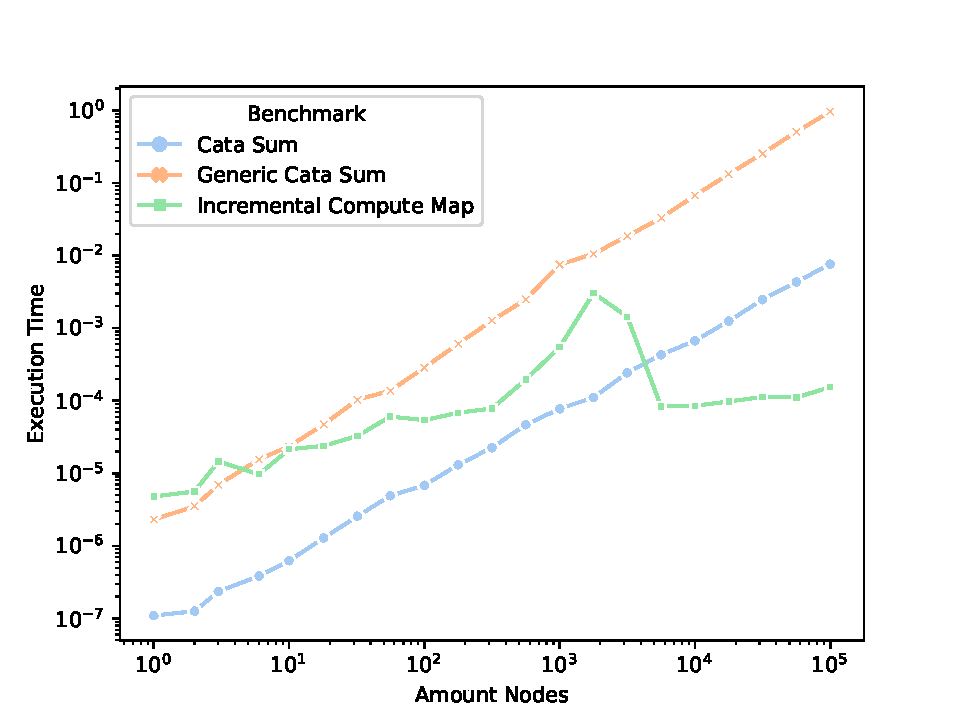
\includegraphics[width=.6\textwidth]{plots/run-2/time/all_benchmarks.pdf}
%     \caption{Overview execution time}
%     \label{fig-exec-time-overview}
% \end{figure}

% \begin{figure}[H]
%     \centering
%     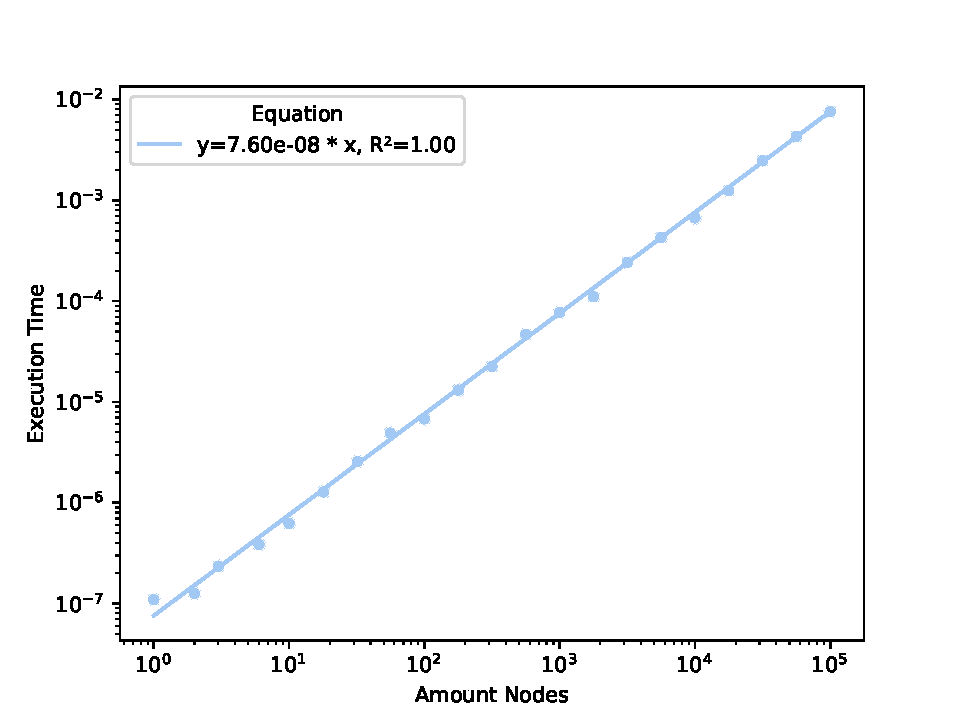
\includegraphics[width=.6\textwidth]{plots/run-2/time/benchmark_cata_sum.pdf}
%     \caption{Execution time for Cata Sum}
%     \label{fig-exec-time-cata-sum}
% \end{figure}

% \begin{figure}[H]
%     \centering
%     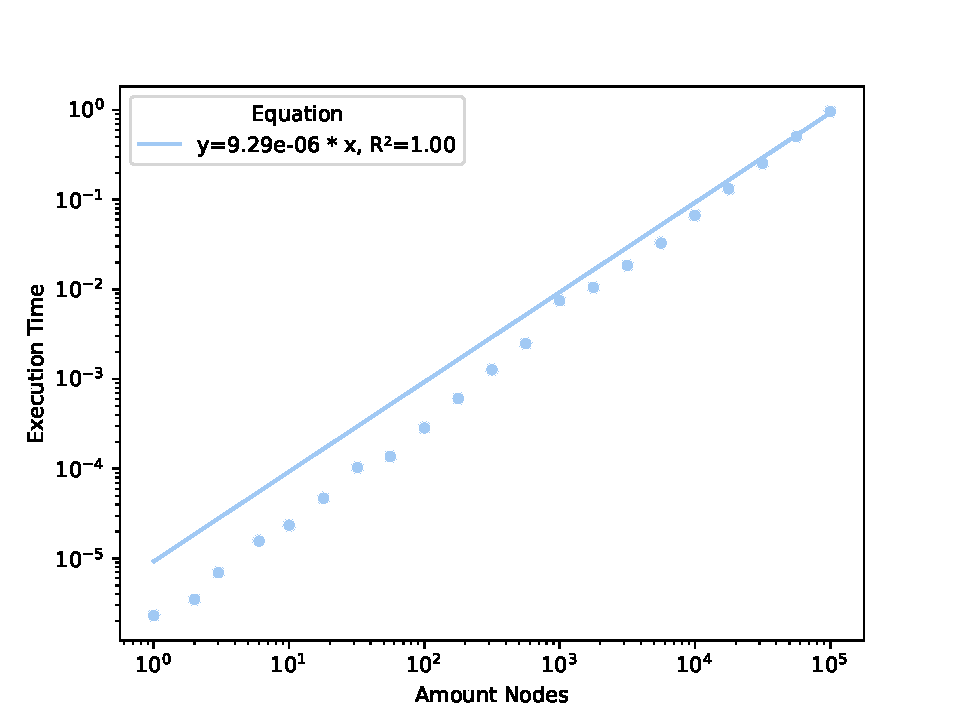
\includegraphics[width=.6\textwidth]{plots/run-2/time/benchmark_generic_cata_sum.pdf}
%     \caption{Execution time for Generic Cata Sum}
%     \label{fig-exec-time-gen-cata-sum}
% \end{figure}

% \begin{figure}[H]
%     \centering
%     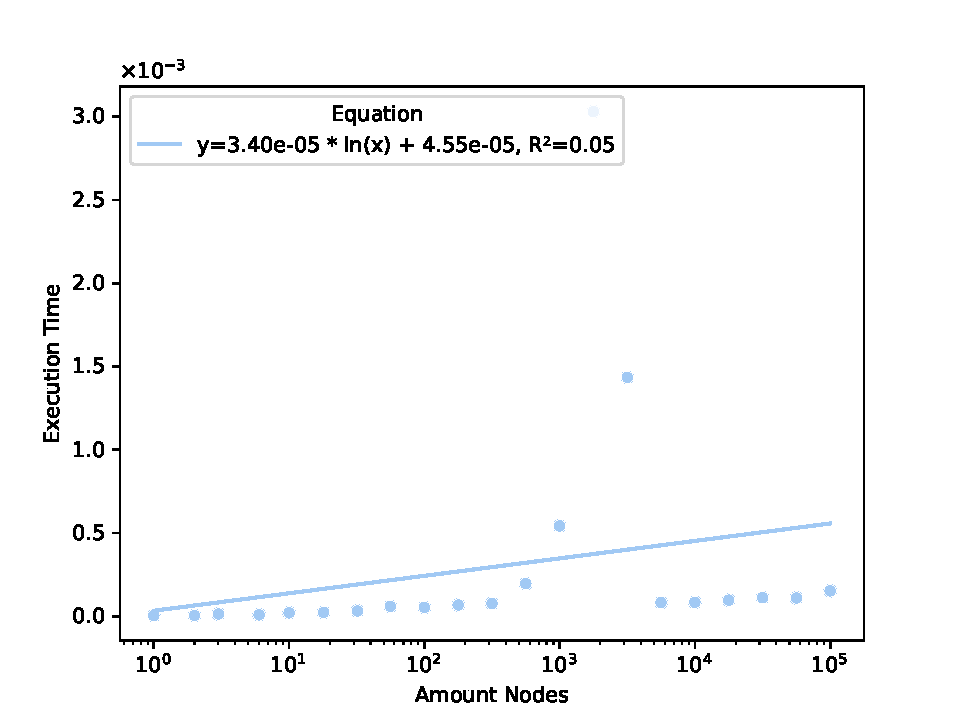
\includegraphics[width=.6\textwidth]{plots/run-2/time/benchmark_incremental_cata_sum.pdf}
%     \caption{Execution time for Incremental Cata Sum}
%     \label{fig-exec-time-inc-cata-sum}
% \end{figure}


\section{Memory Usage}
% \begin{figure}[H]
%     \centering
%     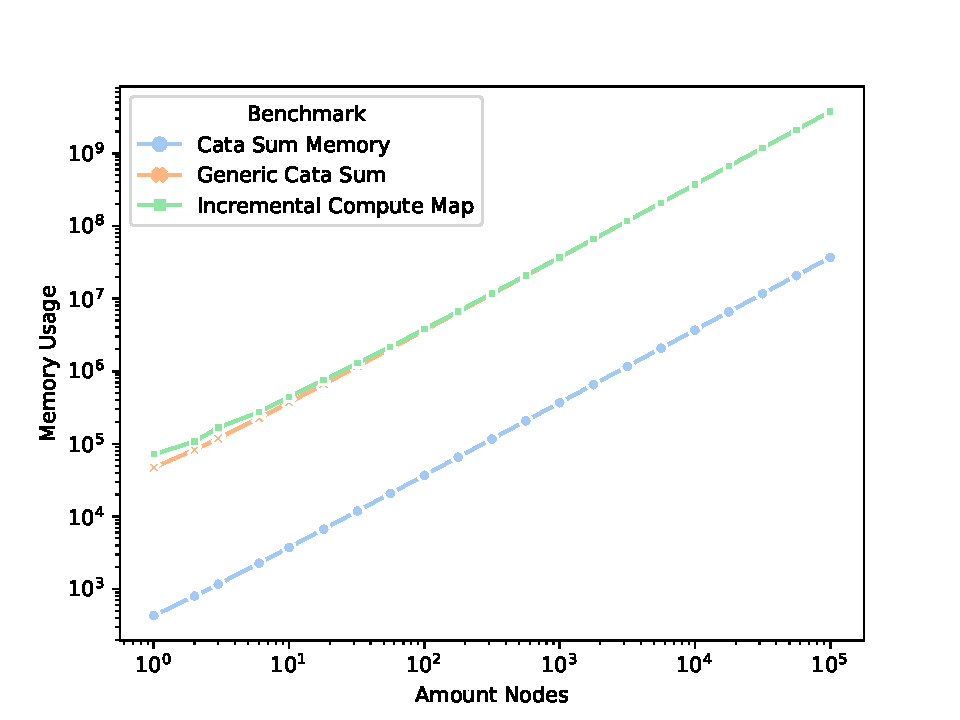
\includegraphics[width=.6\textwidth]{plots/run-2/memory/all_benchmarks.pdf}
%     \caption{Overview memory usage}
%     \label{fig-bytes-all-overview}
% \end{figure}

% \begin{figure}[H]
%     \centering
%     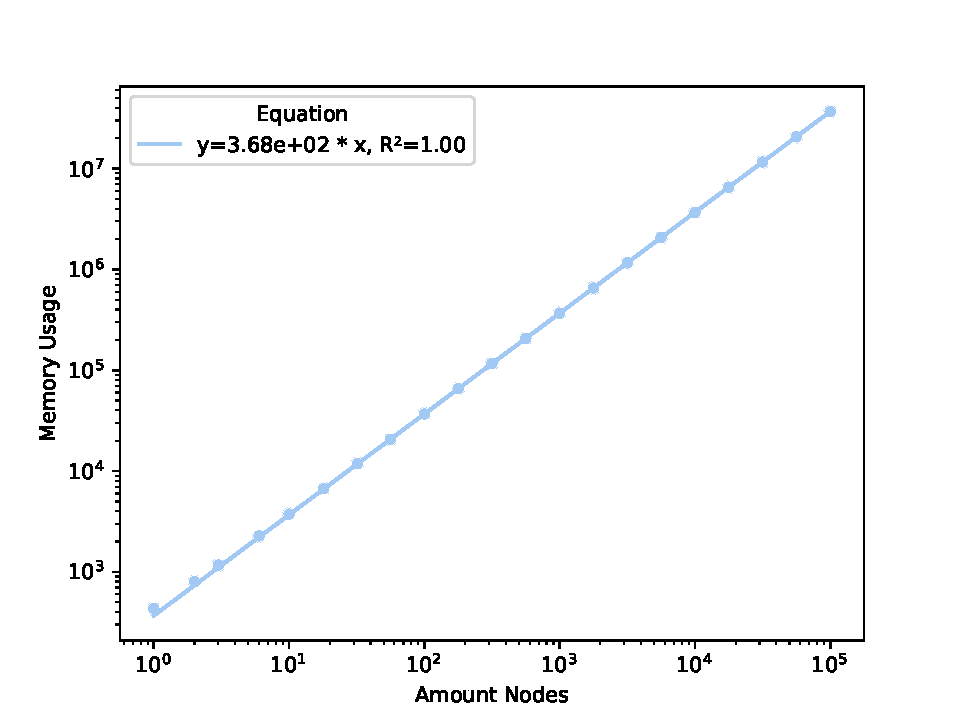
\includegraphics[width=.6\textwidth]{plots/run-2/memory/benchmark_cata_sum.pdf}
%     \caption{Memory usage for Cata Sum}
%     \label{fig-bytes-all-cata-sum}
% \end{figure}

% \begin{figure}[H]
%     \centering
%     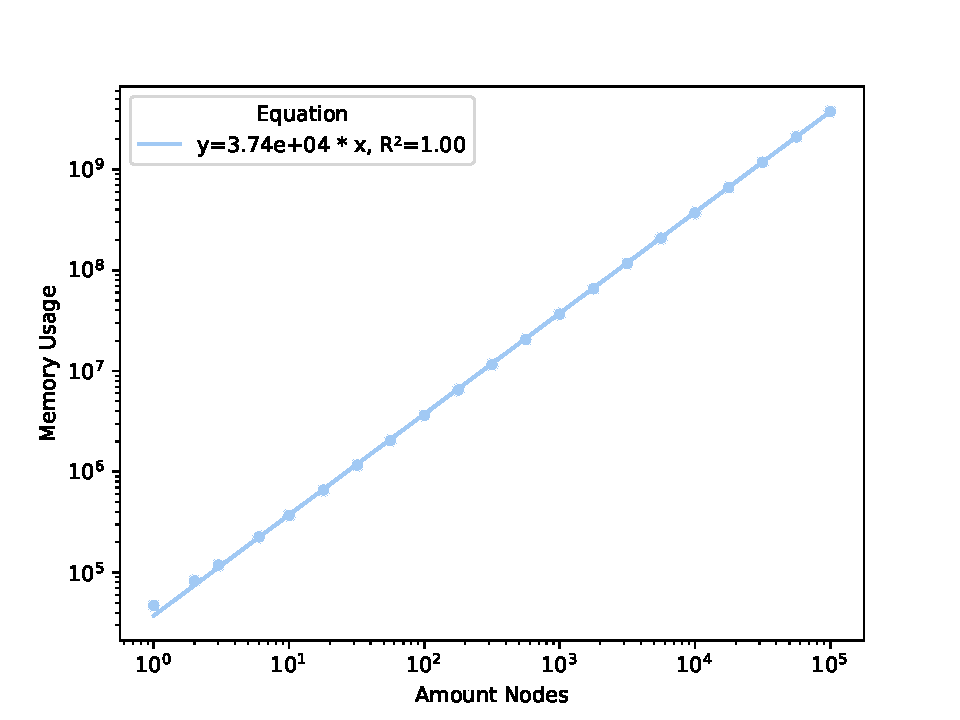
\includegraphics[width=.6\textwidth]{plots/run-2/memory/benchmark_generic_cata_sum.pdf}
%     \caption{Memory usage for Generic Cata Sum}
%     \label{fig-bytes-all-gen-cata-sum}
% \end{figure}

% \begin{figure}[H]
%     \centering
%     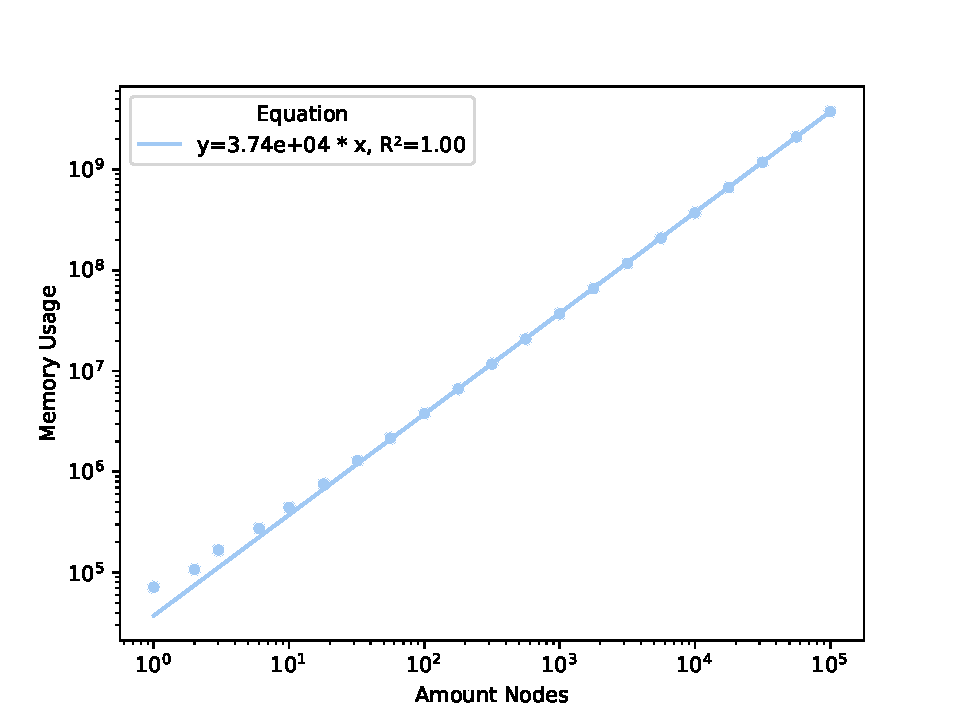
\includegraphics[width=.6\textwidth]{plots/run-2/memory/benchmark_incremental_cata_sum.pdf}
%     \caption{Memory usage for Incremental Cata Sum}
%     \label{fig-bytes-all-inc-cata-sum}
% \end{figure}

\section{Comparison Memory Strategies}
% \begin{figure}[H]
%     \centering
%     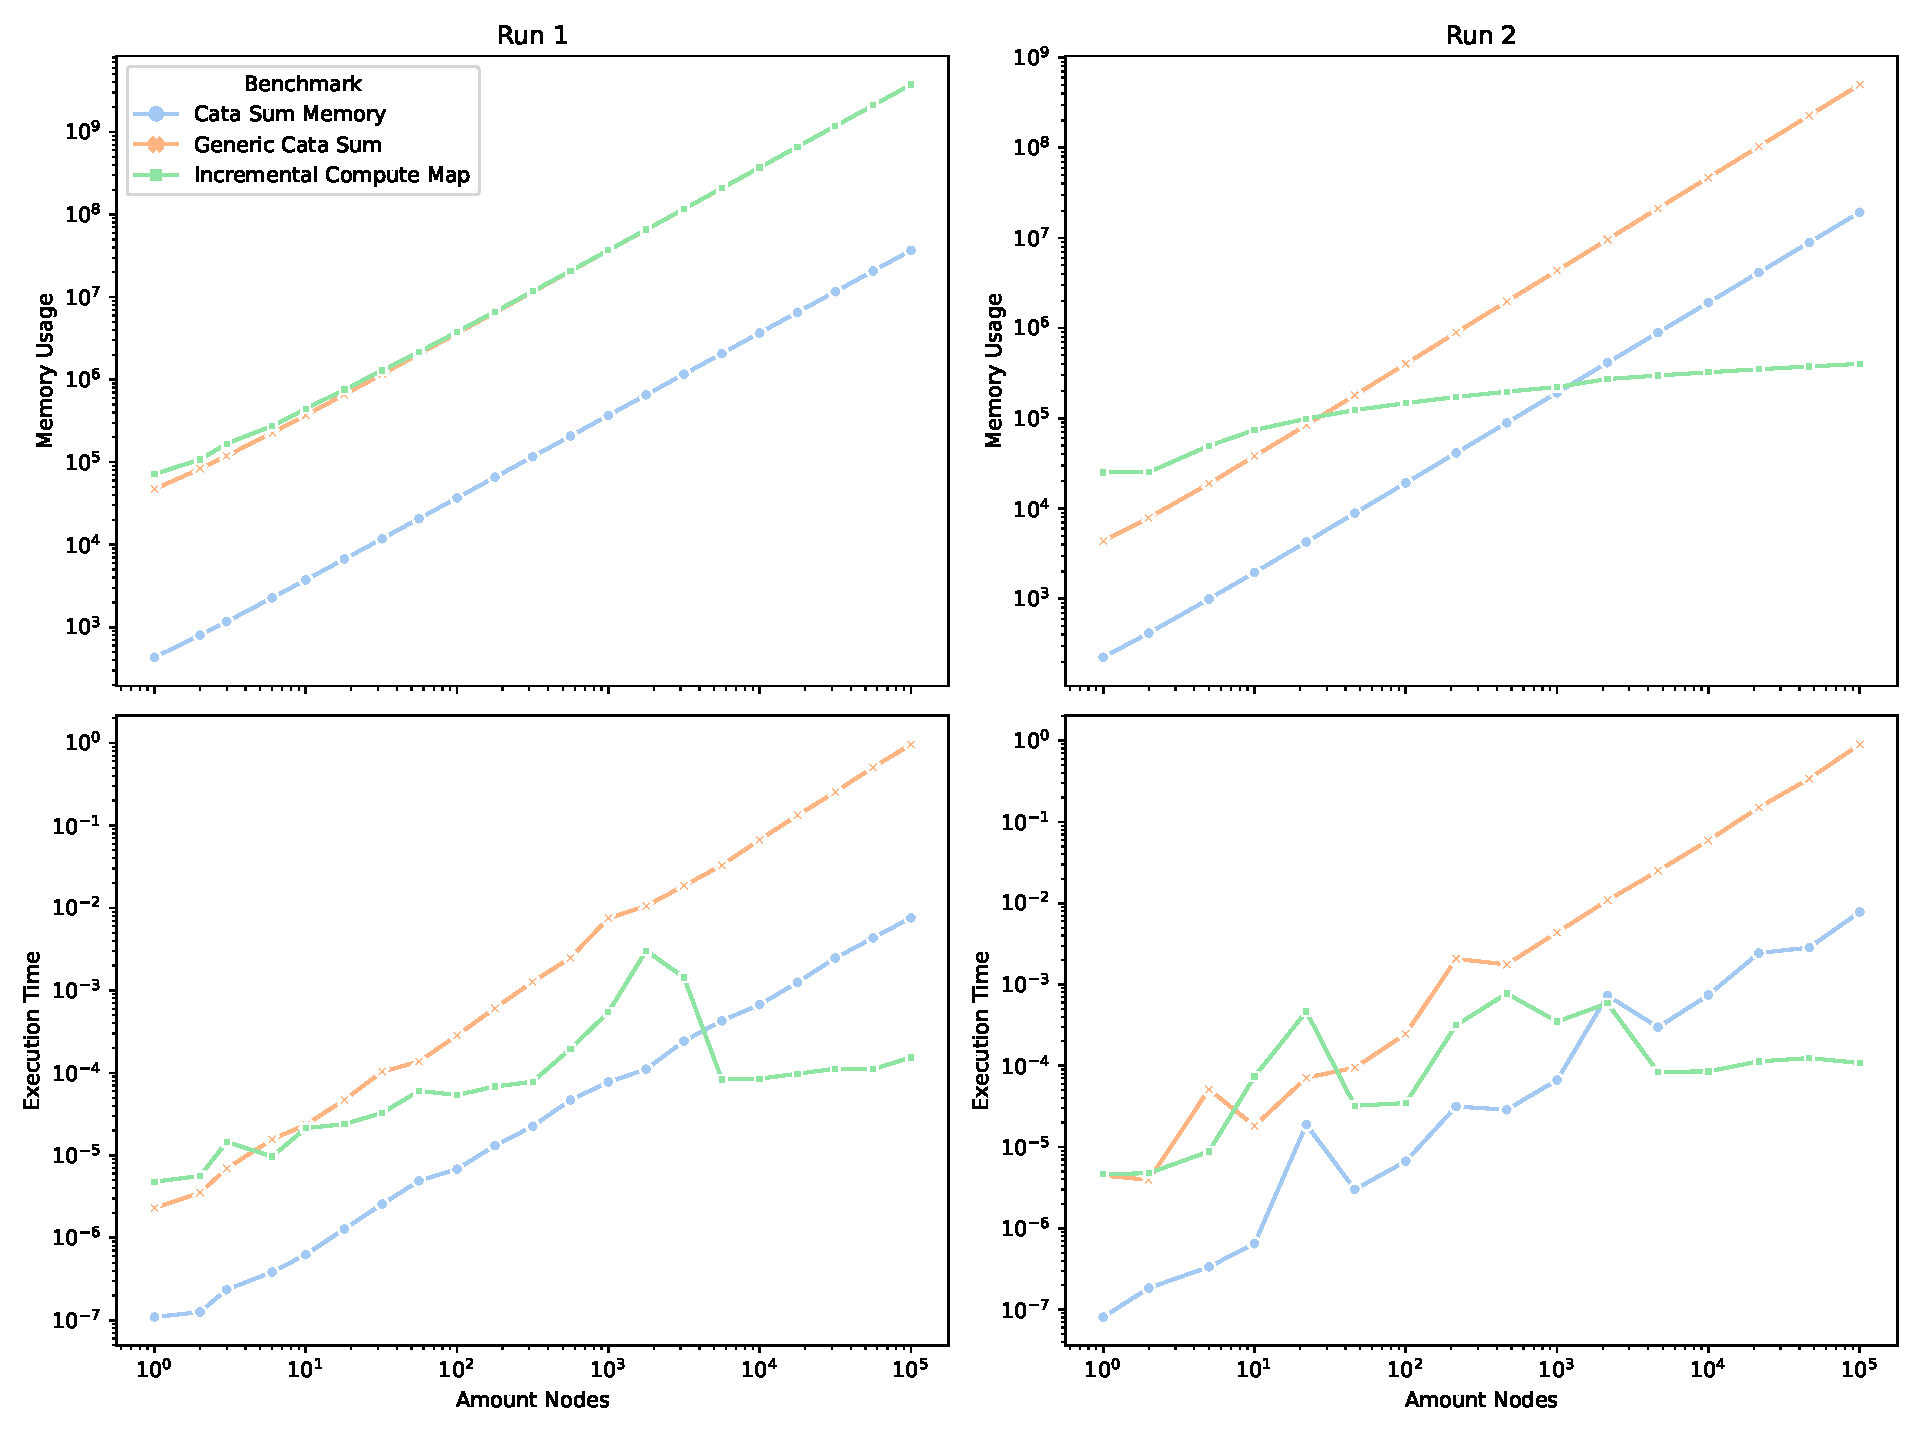
\includegraphics[width=.9\textwidth]{plots/run-2_run-1/comparison_benchmarks.pdf}
%     \caption{Comparison Memory Strategy}
%     \label{fig-comp-mem-strat}
% \end{figure}

\newpage
\chapter{Conclusion}

The results show that the incremental computation is faster, than the non-incremental computation after $10^3$ nodes. However, the initial pass of the incremental computation is slower than the non-incremental computation. Therefore, the optimal use case for the incremental computation is one where there are a lot of small updates to the data structure. This can be accomplished with almost no additional code implemented by the user. 

Furthermore, the additional memory overhead needed for keeping track of all the intermediate results is relatively low. This makes the use of the incremental computation not require a system with additional memory available compared to using the non-incremental computation. 

Nonetheless, if memory usage becomes an issue overtime. A cache replacement policy can be chosen to be used. 

\todo[inline]{Write overview which cache policy replacement for which use case}

\section{Future work}
\todo[inline]{Write future work}

\begin{itemize}
  \item Only results for a sum over data structure computation (no real-world results / only synthetic results)
  \item Only support regular datatypes (not mutually recursive datatypes)
  \item Does not use Sums-of-Products
  \item 
\end{itemize}

\newpage
\section{Appendix}
\appendix

\section{Implementation Memo Cata}

\subsection{Definition Generic Datatypes}
\label{app-def-generic-datatypes}
\begin{minted}{haskell}
data U r         = U
data I r         = I r                  
data K a r       = K a                  
data (:+:) f g r = L (f r) | R (g r)
data (:*:) f g r = (f r) :*: (g r) 
data C c f r     = C (f r)

newtype Fix f = In { out :: f (Fix f) }
\end{minted}

\subsection{Implementation Hashable}
\label{app-impl-hashable}
\begin{minted}{haskell}
class Hashable f where
  hash :: f (Fix (g :*: K Digest)) -> Digest

instance Hashable U where
  hash _ = digest "U"

instance (Show a) => Hashable (K a) where
  hash (K x) = digestConcat [digest "K", digest x]

instance Hashable I where
  hash (I x) = digestConcat [digest "I", getDigest x]
    where
      getDigest :: Fix (f :*: K Digest) -> Digest
      getDigest (In (_ :*: K h)) = h

instance (Hashable f, Hashable g) => Hashable (f :+: g) where
  hash (L x) = digestConcat [digest "L", hash x]
  hash (R x) = digestConcat [digest "R", hash x]

instance (Hashable f, Hashable g) => Hashable (f :*: g) where
  hash (x :*: y) = digestConcat [digest "P", hash x, hash y]

instance (Hashable f) => Hashable (C c f) where
  hash (C x) = digestConcat [digest "C", hash x]
\end{minted}

\subsection{Implementation Merkle}
\label{app-impl-merkle}
\begin{minted}{haskell}
type Merkle f = Fix (f :*: K Digest)

merkleG :: Hashable f 
        => f (Fix (g :*: K Digest)) 
        -> (f :*: K Digest) (Fix (g :*: K Digest))
merkleG f = f :*: K (hash f)

merkle :: (Regular a, Hashable (PF a), Functor (PF a)) 
       => a -> Merkle (PF a)
merkle = In . merkleG . fmap merkle . from
\end{minted}

\subsection{Implementation Cata Merkle}
\label{app-impl-cata-merkle}
\begin{minted}{haskell}
cataMerkleState :: (Functor f, Traversable f)
                => (f a -> a) -> Fix (f :*: K Digest) 
                -> State (M.Map Digest a) a
cataMerkleState alg (In (x :*: K h)) = do m <- get
  case M.lookup h m of
    Just a -> return a
    Nothing -> do y <- mapM (cataMerkleState alg) x
                  let r = alg y
                  modify (M.insert h r) >> return r

cataMerkle :: (Functor f, Traversable f)
           => (f a -> a) -> Fix (f :*: K Digest) -> (a, M.Map Digest a)
cataMerkle alg t = runState (cataMerkleState alg t) M.empty
\end{minted}

\subsection{Implementation Zipper Merkle}
\label{app-impl-zipper-merkle}
\begin{minted}{haskell}
data Loc :: * -> * where
  Loc :: (Zipper a) => Merkle a 
                    -> [Ctx (a :*: K Digest) (Merkle a)] 
                    -> Loc (Merkle a)

modify :: (a -> a) -> Loc a -> Loc a
modify f (Loc x cs) = Loc (f x) cs

updateDigest :: Hashable a => Merkle a -> Merkle a
updateDigest (In (x :*: _)) = In (merkleG x)

updateParents :: Hashable a => Loc (Merkle a) -> Loc (Merkle a)
updateParents (Loc x []) = Loc (updateDigest x) []
updateParents (Loc x cs) = updateParents
                          $ expectJust "Exception: Cannot go up"
                          $ up (Loc (updateDigest x) cs)

updateLoc :: Hashable a => (Merkle a -> Merkle a) 
                        -> Loc (Merkle a) -> Loc (Merkle a)
updateLoc f loc = if   top loc'
                  then loc'
                  else updateParents 
                       $ expectJust "Exception: Cannot go up" (up loc')
  where
    loc' = modify f loc
\end{minted}

\section{Regular}

\subsection{Zipper}
\begin{minted}{haskell}
data instance Ctx (K a) r
data instance Ctx U r
data instance Ctx (f :+: g) r = CL (Ctx f r) | CR (Ctx g r)
data instance Ctx (f :*: g) r = C1 (Ctx f r) (g r) | C2 (f r) (Ctx g r)
data instance Ctx I r = CId
data instance Ctx (C c f) r = CC (Ctx f r)
data instance Ctx (S s f) r = CS (Ctx f r)
\end{minted}

\newpage
\printbibliography

\end{document}